\subsection{Slant Incident HWP properties}

\paragraph{Description:}
At non-normal incidence, the HWP optical properties change. This effect is small for angles $<$10 degrees away from the normal incidence and increases for larger angular deviations. Stray light, instrumental emissions and reflections can produce off-axis radiation crossing and reflecting the HWP.

\textbf{What systematics do these contribute to?} The general result of slant incidence effects is to change the phase delay and the amplitude of the 2$\,f$ and 4$\,f$ signals; any approach consisting in measuring/estimating these signals under normal incidence hypothesis and subtract from the data as template, might not be reliable. 

\subsubsection{Birefringent HWP}\label{slant_biri}

\paragraph{Plan to model and/or measure:}
For a birefringent HWP, how the optical properties change with the incidence angle can be modeled if you know the optical properties of the birefringent material as a function of frequency and include the AR coating. This can be estimated with numerical simulations and crystallography properties. Fourier Trasform Spectrometer (FTS) and reflectometery measurements with the angle of incoming light at different, non-normal, incident angles with respect to the HWP can be used to measure the dependence of the optical properties as a function of the incident angle.

\textbf{Using the modeled/measured values, how do we model the impact of this response on the science?}
These measurements can be used to build the Mueller matrix under slant incident incoming radiation. Fig.~\ref{fig:Sa_elements} shows the Mueller matrix elements $M_{ij}$ in transmission of a single-layer HWP optimized for $150\,\mathrm{GHz}$. The behaviour of the elements is shown as a function of the HWP rotation angle $\chi$ in the case of normal incidence (blue curve), at $10^\circ$-incidence (orange) and at $20^\circ$-incidence (green). To highlight the small deviation of slant incidence from the case of normal incidence, the right panel of Fig.~\ref{fig:Sa_elements} reports the difference between $M_{ij}$ at slant incidence and $M_{ij}$ at normal incidence.  

An alternative approach to model the behaviuor at slant incidence would be to directly measure the HWP Mueller matrix components studying the output signal from an unpolarized and totally polarized incoming radiation crossing the HWP and followed by a fixed polarizer. The measurement should be performed for dfferent frequency values, to reconstruct the spectral trend of the components: see for example Figs.\,5 and 6 in \cite{Salatino17} which demonstrate how these trends change with respect to the incidence angle of the incoming radiation. The simulated trend of Fig.\,5 in \cite{Salatino17} agrees well with the ones measured from the Spider HWP \cite{Bryan10}.


This effect is not modeled in the literature, and could be large in some cases, so the SRF is 4.

\paragraph{Uncertainty/Range:}
In most cases the optical properties (refraction indices, absorption angle) come from literature, so there is some uncertainty in the parameters from the variation between batches of materials. However, the main source of uncertainty comes from uncertainty in understanding how these optical properties, generally measured at room temperature, scale to cryogenic temperatures.

\textbf{Include how big the science impacts can be for this within SO.}

\paragraph{Parameterization:}
Analytically, this effect can be estimated building the Mueller matrix of the birifringent HWP considering how the refraction index along the extraordinary axis depends on the incidence angle, $i$:
\begin{equation}
%n(i)=((\frac{\cos{i}}{n_e(\nu))^2}+(\frac{\sin{i}}{n_o(\nu)})^2)^{(-0.5)};
n(i)=n_e\sqrt{1+(n_e^{-2}(\nu)-n_o^{-2}(\nu))n_1^2\sin^2(i)\cos^2(\chi)};
\end{equation}
where $n_e(\nu)$ ($n_o(\nu)$) are the extraordinary (ordinary) refraction index, $\nu$ is the frequency of the incoming radiation, $n_1$ is the index of refraction of the medium where the incoming radiation propagates ($n_1=1$ as we usually assume air), and $\chi$ is the HWP rotation angle. \textbf{How do we parametrize the science impact}

From both the analytical approach and the experimental one (i.e. reconstruction of the Mueller matrix components from the measurement described above), the amplitude of the resulting 2$\,f$ and 4$\,f$ signals, i.e. $A_2$ and $A_4$, can be estimated as:

\begin{eqnarray}
  A_2 &=& \int_{\Delta\nu} \frac{I(\nu)+Q(\nu)}{2} \rho(\nu) d\nu\\ \label{A2}
  A_4 &=& \int_{\Delta\nu} \frac{t(\nu)-c(\nu)}{4} Q(\nu) d\nu; \label{A4}
\end{eqnarray}
where $I(\nu)$ and $Q(\nu)$ is the Stokes vector of the incoming radiation (here as an example we assumed to be $(I(\nu), Q(\nu),0,0)$),
$\rho(\nu), t(\nu)$ and $c(\nu)$ the Mueller matrix components (eq.\,\ref{eq:Mueller_Matrix}). The spectral trend of all the involved quantities is integrated on a given HWP band $\Delta\nu$. A more generic approach to quantify the coefficients $A_2$ and $A_4$ is detailed in Sec.~\ref{IP downstream of HWP}.

\begin{figure}
\centering
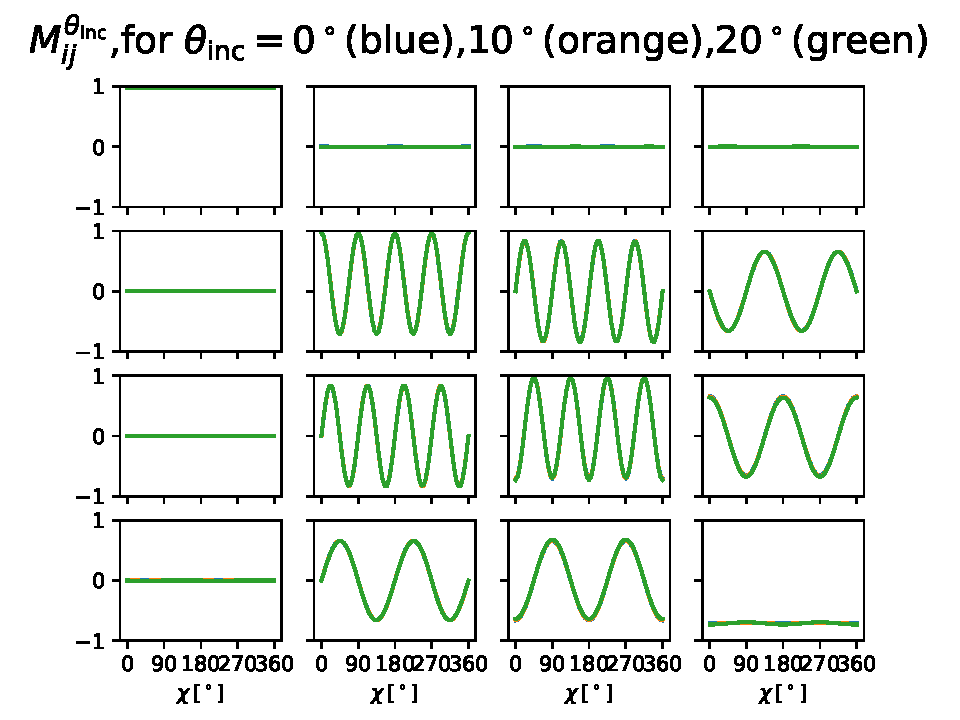
\includegraphics[width=0.5\linewidth]{figures/Mueller_elements_0_10_20deg.pdf}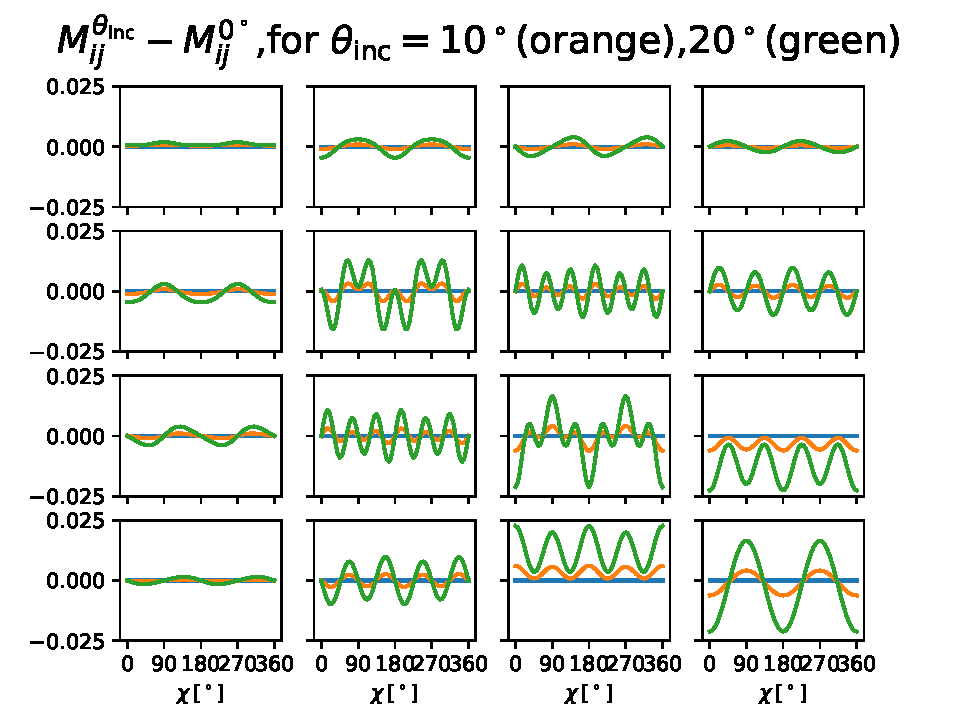
\includegraphics[width=0.5\linewidth]{figures/Mueller_elements_diff.pdf}
\caption{Left panel: Mueller matrix components $M_{ij}$ in transmission as a function of the HWP rotation angle $\chi$. The components are for a real Sapphire HWP
optimized for 150 GHz (with AR coating). We have considered three incidence angles: $\theta_\mathrm{inc}=0^\circ$ (blue), $\theta_\mathrm{inc}=10^\circ$ (orange), and $\theta_\mathrm{inc}=20^\circ$ (green). Right panel: To highlight the small deviation of the behaviour of the HWP from the case of normal incidence, the difference between Mueller matrix components at non-normal incidence and the Mueller matrix components at $0^\circ$-incidence are shown as a function of the rotation angle $\chi$.
}\label{fig:Sa_elements}
\end{figure}

%\begin{figure}
%\centering
%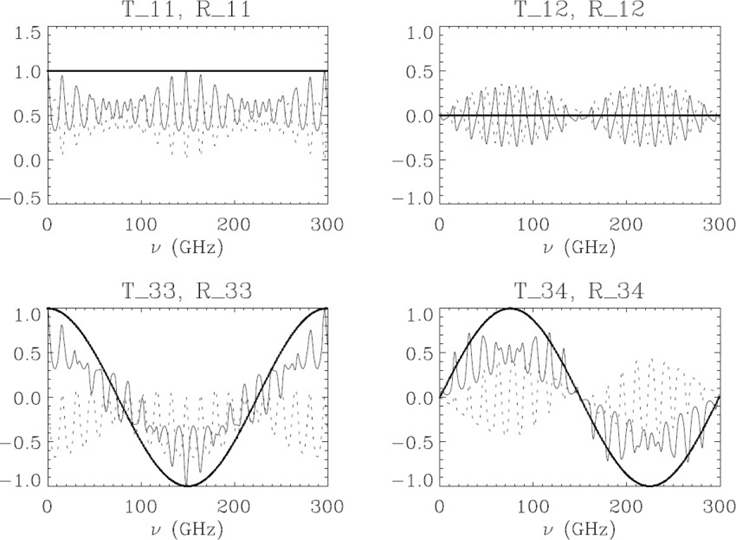
\includegraphics[width=0.6\linewidth]{figures/0deg.png}
%\caption{Mueller matrix components, for both transmission (T) and reflection (R), of a real Sapphire HWP
%optimized for 150 GHz (no AR coating). The incoming radiation is at normal incidence \cite{Salatino17}.
%}\label{0deg}
%\end{figure}

%\begin{figure}
%\centering
%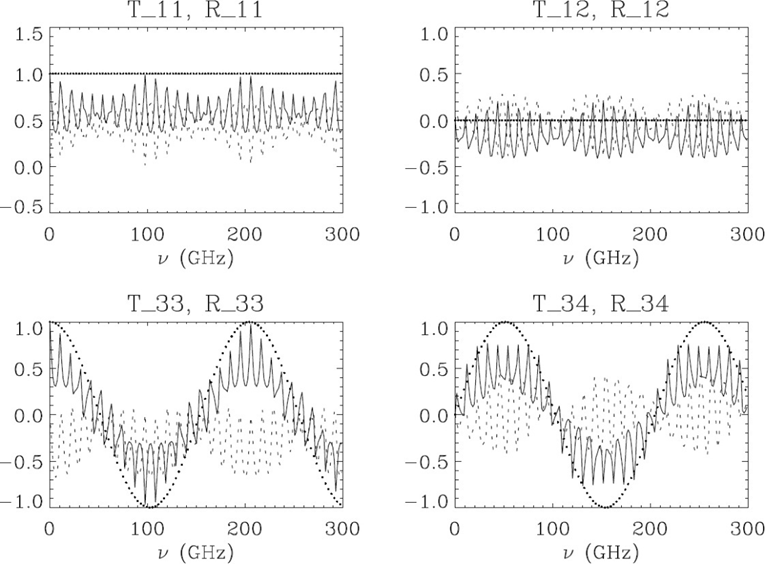
\includegraphics[width=0.6\linewidth]{figures/45deg.png}
%\caption{Mueller matrix components, for both transmission (T) and reflection (R), of a real Sapphire HWP
%optimized for 150 GHz (no AR coating). The incoming radiation is at 45deg incidence \cite{Salatino17}.}\label{45deg}
%\end{figure}

%------------------------
\subsubsection{Metamaterial HWP}

\begin{figure}
\centering
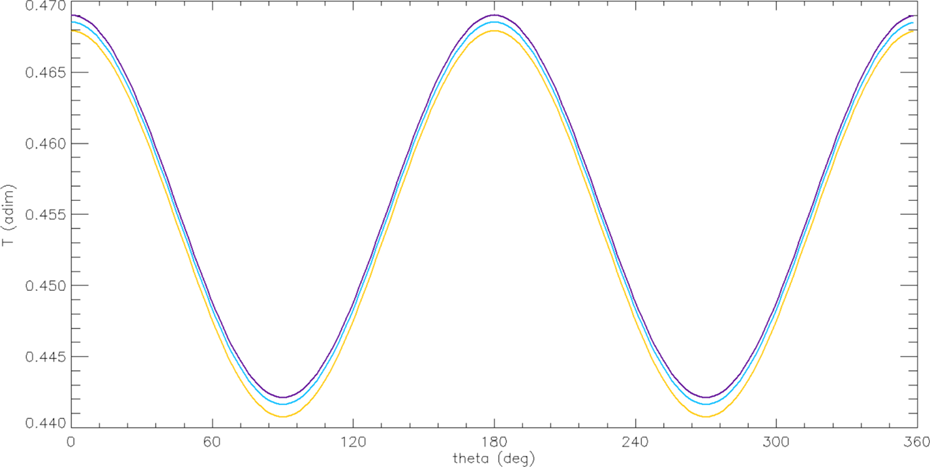
\includegraphics[width=0.6\linewidth]{figures/meta1.png}
\caption{Simulated output signal (dimensionless units) at 70GHz from an unpolarized radiation crossing the AdvACT MF metamaterial HWP. The HWP is %optimized for a frequency band centered
on 90 GHz. Violet line: -10deg, cyan line 0deg and orange 10deg incident angle. At 10deg away from the normal incidence, the output %signal
changes by 0.03.}\label{meta1}
\end{figure}

\begin{figure}
\centering
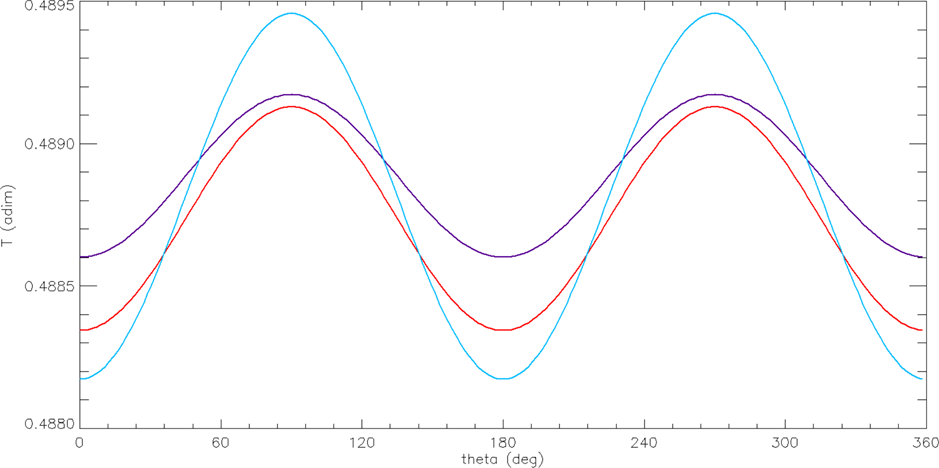
\includegraphics[width=0.6\linewidth]{figures/meta2.png}
\caption{Simulated output signal (dimensionless units) at 90GHz from an unpolarized radiation crossing the AdvACT MF metamaterial HWP. The HWP is %optimized for a frequency band centered
on 90 GHz. Violet line: -10deg, red line 0deg and cyan 10deg incident angle. At 10deg away from the normal incidence, the output signal
changes by 0.0015.}\label{meta2}
\end{figure}

\paragraph{Plan to model and/or measure:}
For a metamaterial HWP, uderstanding of how the optical properties change with the incident angle requires simulations in HFSS or CST. HFSS simulations have demonstrated that the variation in the output signal increases at frequencies closest to the central working frequency of the
HWP (Figs. \ref{meta1} and \ref{meta2}). 
Like the birefringent case, FTS and reflectometry measurements can provide experimental estimates of the optical properties.

\textbf{Using the modeled/measured values, how do we model the impact of this response on the science?}

This effect is not modeled in the literature, and could be large in some cases, so the SRF is 4.

\paragraph{Uncertainty/Range:}
\textbf{Add info here as it becomes available.}

\paragraph{Parameterization:}
HFSS/CST simulations can give the optical properties as a function of the incident angle $i$. \textbf{How do we parametrize the science impact} From these, the Mueller matrix for slant incident angle can be build and the amplitude of the $2\,f$ and $4\,f$ signals estimated as described for the birifringent HWP (Sec.\,\ref{slant_biri}). 
